\documentclass[twoside]{article}

%\usepackage{graphics}
\usepackage{graphicx}


\usepackage[sc]{mathpazo} % Use the Palatino font
\usepackage[T1]{fontenc} % Use 8-bit encoding that has 256 glyphs
\linespread{1.05} % Line spacing - Palatino needs more space between lines
\usepackage{microtype} % Slightly tweak font spacing for aesthetics

\usepackage[hmarginratio=1:1,top=32mm,columnsep=20pt]{geometry} % Document margins
\usepackage{multicol} % Used for the two-column layout of the document
%\usepackage{nonfloat}
\usepackage{float}
\usepackage{tikz}
\usepackage{amsmath}

\usepackage[hang, small,labelfont=bf,up,textfont=it,up]{caption} % Custom captions under/above floats in tables or figures
\usepackage{booktabs} % Horizontal rules in tables
\usepackage{float} % Required for tables and figures in the multi-column environment - they need to be placed in specific locations with the [H] (e.g. \begin{table}[H])
\usepackage{hyperref} % For hyperlinks in the PDF

\usepackage{lettrine} % The lettrine is the first enlarged letter at the beginning of the text
\usepackage{paralist} % Used for the compactitem environment which makes bullet points with less space between them

\usepackage{makecell} %table cells
\usepackage{booktabs} %table appearance

\usepackage{abstract} % Allows abstract customization
\renewcommand{\abstractnamefont}{\normalfont\bfseries} % Set the "Abstract" text to bold
\renewcommand{\abstracttextfont}{\normalfont\small\itshape} % Set the abstract itself to small italic text

\usepackage{titlesec} % Allows customization of titles
\usepackage[utf8]{inputenc}

\renewcommand{\thesection}{\Roman{section}} 
\renewcommand{\thesubsection}{\thesection.\Roman{subsection}}


\titleformat{\section}[block]{\large\scshape\centering}{\thesection.}{1em}{} % Change the look of the section titles
\titleformat{\subsection}[block]{\large}{\thesubsection.}{1em}{} % Change the look of the section titles


%%%%%%%%%%%%%%%%%%
%%% Table Box 

\def\boxit#1#2{%
	\smash{\color{#1}\fboxrule=1pt\relax\fboxsep=2pt\relax%
		\llap{\rlap{\fbox{\vphantom{0}\makebox[#2]{}}}~}}\ignorespaces
}


%----------------------------------------------------------------------------------------
%	TITLE SECTION
%----------------------------------------------------------------------------------------

\title{\vspace{-15mm}\fontsize{24pt}{10pt}\selectfont\textbf{Wine Quality Prediction on the UCI Wine Dataset}} % Article title 

\author{
	\large
	\textsc{Massimiliano Pronesti}\\[2mm] % Your name
	\normalsize Politecnico di Torino \\ % Your institution
	\normalsize \href{mailto:s287646@studenti.polito.it}{s287646@studenti.polito.it} % Your email address
	\vspace{-5mm}
}
\date{}

%----------------------------------------------------------------------------------------

\begin{document}
	
	\maketitle % Insert title
	\begin{abstract}
    \noindent This report provides an analysis of the effectiveness of different classification approaches applied to the popular wine quality prediction problem on the wine dataset from the UCI repository. Specifically, the goal is to predict whether the wine has a good or a bad quality. The original dataset consists of 10 classes. Nevertheless, for this work, the dataset has been binarized, collecting all wines with low quality (lower than 6) into class 0, and good quality (greater than 6) into class 1, while those with quality 6 have been discarded.
    In addition, the dataset contains both red and white wines (merged for the sake of this analysis). There are 11 features, that represent physical properties of the wine, with partially balanced classes.
\end{abstract}

	\begin{multicols}{2} % Two-column layout throughout the main article text
		\section{Data Analysis}

\lettrine[nindent=0em,lines=3]{I}n this section, we are going to conduce an analysis on the main characteristics of the features contained in the training dataset. The training set consists of 1126 bad quality samples and 613 good quality samples, then one class is twice as much present as the other. A visualization of how raw features are distributed is shown in Figure \ref{fig:raw}.

\begin{figure}[H]
	\foreach \i in {0,1,...,10}{
		\includegraphics[width=.15\textwidth]{assets/raw_hist\i}
	}
\caption{Raw features distribution of the UCI Wine Quality Dataset}
\label{fig:raw}
\end{figure}

We can observe that features don't have a zero mean, therefore we might consider standardizing them, i.e. centering data and scaling it by the variance, so that the obtained random variable has zero mean and unitary variance. 

In addition, features don't expose a Gaussian trend, with the presence of some outliers.

Therefore, we gaussianize the features, computing the cumulative rank $r(x)$ over the training set 
\begin{align*}
	r(x) = \frac{\sum^N_{i=1} I[x < x_i] + 1}{N + 2}
\end{align*}

being $x_i$ the value of the considered feature for the i-th sample, and transforming the features computing the inverse of the cumulative distribution function $\Phi$ fed with the rank $r(x)$

\begin{align*}
	X_{gauss} = \Phi^{-1} (r(x)) 
\end{align*}

The distribution of the gaussianized features is shown in Figure \ref{fig:gauss}.


Moreover, we provide an analysis of the correlation between the features, exploiting the Pearson product-moment correlation coefficient, defined as

\begin{align*}
	\rho_{X, Y} = \frac{cov(X, Y)} {\sigma_X \sigma_Y}
\end{align*}


\begin{figure}[H]
	\foreach \i in {0,1,...,10}{
		\includegraphics[width=.15\textwidth]{assets/gauss_hist\i}
	}
	\caption{Gaussianized features distribution of the UCI Wine Quality Dataset}
	\label{fig:gauss}
\end{figure}

being $cov(X, Y)$ the covariance matrix of $X$ and $Y$, expressible as the expectation of the product of $X$ and $Y$ centered using their respective mean.

\begin{align*}
	cov(X, Y) = \mathbb{E}[(X - \mu_X)(Y - \mu_Y)]
\end{align*}

The obtained heatmaps among the gaussianized features are shown in Figure \ref{fig:heat}.

\begin{figure}[H]
	\begin{minipage}{\textwidth}
	\hspace{-.2cm}
	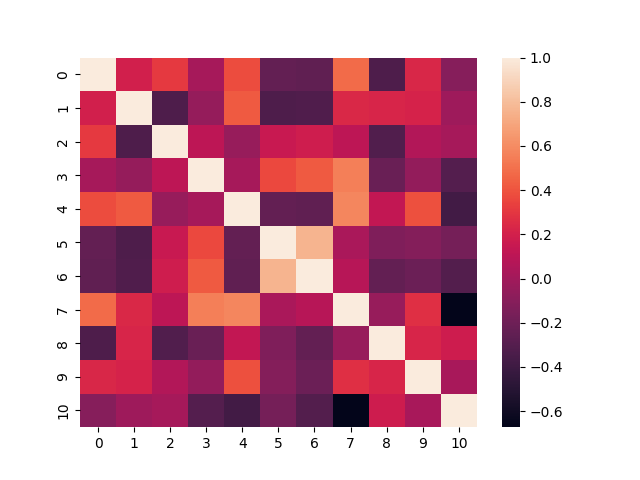
\includegraphics[width=.17\textwidth]{assets/gauss_feat_heat}
	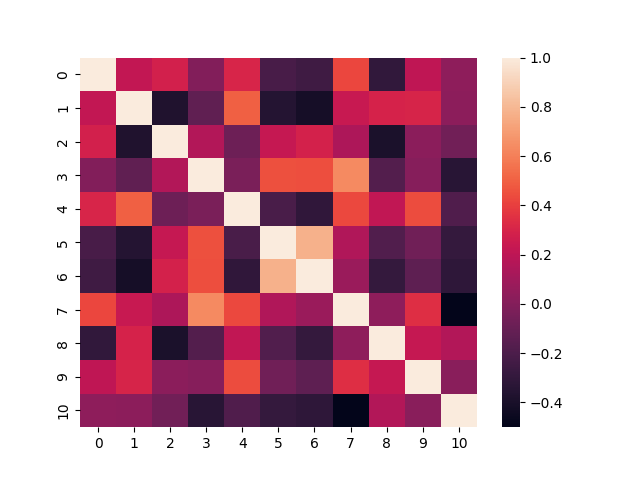
\includegraphics[width=.17\textwidth]{assets/gauss_feat_heat0}
	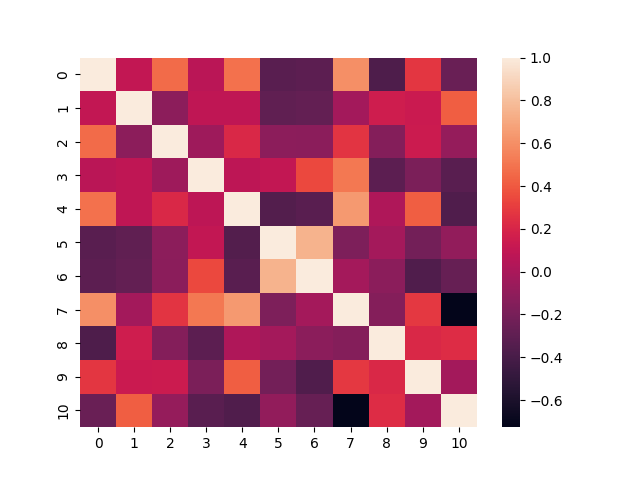
\includegraphics[width=.17\textwidth]{assets/gauss_feat_heat1}
	\end{minipage}

	\caption{Heatmaps among Gaussianized features}
	\label{fig:heat}	
\end{figure}

where we can observe some features are correlated (darker colors in the heatmap), thus exploring dimensionality reduction techniques such as the PCA, could prove beneficial.
				\section{Methods}
Actualmente existen varios tipos de Barómetros. Según los fines del instituto o experimento a realizarse uno es ocupado o no, así mismo, la tecnología y el presupueto disponible, varía su construcción y manufactura. A continuación los nombramos:\\


\begin{compactitem}
	\item Barómetro de Mercurio:
	Está formado por un tubo de vidrio de unos 850 mm de altura, cerrado por elextremo superior y abierto por el inferior. Cuando el tubo se llena de mercurio yse coloca el extremo abierto en un recipiente lleno del mismo líquido, el niveldel tubo cae hasta una altura de unos 760 mm por encima del nivel delrecipiente y deja un vacío casi perfecto en la parte superior del tubo, estando alnivel del mar y en condiciones normales. Las variaciones de la presiónatmosférica hacen que el líquido del tubo suba o baje ligeramente. La lecturade un barómetro de mercurio puede tener una precisión de hasta 0,1 mm.\\
	
	
	\item Barómetro de Fortín:
	Compuesto por un tubo de Torricelli que se introduce en el mercurio contenido en una cubeta de vidrio en forma tubular, provista de una base de piel de gamo cuya forma puede ser modificada por medio de un tornillo que se apoya en su centro y que, oportunamente girado, lleva el nivel del mercurio del cilindro a rozar la punta de un pequeño cono de marfil. Así se mantiene un nivel fijo.Este está completamente recubierto de latón, salvo dos ranuras verticales junto al tubo que permiten ver el nivel de mercurio. En la ranura frontal hay una graduación en milímetros y una escala de vernier (nonio) para la lectura de décimas de milímetros.Y en la posterior hay un pequeño espejo para facilitar la visibilidad del nivel.Los barómetros Fortin se usan en laboratorios científicos para las medidas de alta precisión.\\
	
	
	\item Barómetro Aneroide:
	Es un barómetro que no utiliza mercurio. Indica las variaciones de presión atmosférica por las deformaciones más o menos grandes que aquélla hace experimentar a una caja metálica de paredes muy elásticas en cuyo interior se ha hecho el vacío más absoluto. Se gradúa por comparación con un barómetro de mercurio pero sus indicaciones son cada vez más inexactas por causa de la variación de la elasticidad del resorte plástico. Fue inventado por Lucien Vidie en 1843 y es más grande, por lo tanto el barómetro que utiliza mercurio. El principio de funcionamiento es el cambio de tamaño de una cápsula parcialmente evacuada, construida para maximizar el cambio en una dimensión con los cambios en la presión del aire. Los cambios de la longitud de la cápsula se amplifican por medio de un brazo a un dial, que permite mostrar la presión.\\
	\
	\item Barómetro Holostérico 
	Está formado por un recipiente aplanado, de superficies onduladas en el que se ha logrado una intensa rarefacción antes de cerrarlo; en una de las caras se apoya un resorte que, con las variaciones de presión atmosférica, hace mover un índice por medio de un juego de palancas.Es menos preciso que el Aneroide.
	
	
	
\end{compactitem}
		\section{Evaluation}

\begin{table}[H]
	\caption{Algunos equipos}
	\centering
	\begin{tabular}{llr}
		\toprule
		\multicolumn{2}{c}{Barómetro} \\
		\cmidrule(r){1-2}
		Equipo & Rango hPa& Precio  \\
		\midrule
		
		Baromería en hPa & 580 - 1040& $998USD$ \\\\
		Registrador bar & 10 – 999.9 & $218USD$ \\\\
		BARÓMET AB60 & 800-1100&$$\\\\
		BARÓMET AB100 &600-1100&\\\\
		VAISALA PTB110 &5,6,8,11 (x100)&\\\\
		\bottomrule
	\end{tabular}
\end{table}

Aquí presentamos mayor detalles de los equipos de la tabla de arriba:\\\\

Barómetro AB 60\\
Fabricante: Ammonit\\
Venta en el interior del armario de conexiones y por separado\\
Sensor de presión piezoeléctrico\\
Intérvalo de medida 800-1100 hPa (mbar)\\
Tensión de salida: 0-5 VDC\\Tensión entrada: 9-32 V\\
Consumo: < 5 mA @ 12 VDC\\
Temperatura de funcionamiento: -40 - 85 C\\
Humedad de funcionamiento: 0-98 po ciento RH\\
Atmósfera: No iónica, no corrosiva\\
Tiempo de respuesta: 10-90 por ciento, typ. 50 ms.\\\\

VAISALA PTB 110\\
Fabricante: Vaisala\\
Intérvalo de medida: 500, 600, 800-1100 hPA\\
Sensor piezoeléctrico: Bajo consumo\\
Medida de diferentes intérvalos
Exactitud:tol.:3 hPa a 20 C;tol.:1 hPa at -20-60 C tol.:1,5 hPa at -40-60 C\\\\
Tensión de salida: 0-2,5 ó 0-5 VDC\\
Consumo: < 4 mA @ 12 VDC\\
		\section{Discussion and Conclusions}






	\end{multicols}
	
\end{document}